\documentclass{sciposter}

\usepackage[brazil]{babel}
\usepackage[utf8]{inputenc}
\usepackage[centertags]{amsmath}
\usepackage{hyperref,amsfonts,multirow,multicol}
\hypersetup{pdfpagelayout=SinglePage}
\usepackage{graphicx,colortbl}
\usepackage{geometry}
\geometry{paperwidth=90cm,paperheight=100cm,centering,
textwidth=77cm,textheight=87cm,left=3cm,top=3cm}
\usepackage{braket}
\usepackage{multicol}
\usepackage{wrapfig}
\pagestyle{plain}
\frenchspacing

%%Definindo cores
\definecolor{BoxCol}{RGB}{44,54,181} %azul

%%Define o caminho das figuras, válido somente para o comando \includegraphics
\graphicspath{{imagens/}}


%%Transformando tudo em branco
\renewcommand{\thesection}{\textcolor{white}{\arabic{section}}}
\renewcommand{\thesubsection}{\textcolor{white}{\arabic{section}.\arabic{subsection}}}
\addto\captionsbrazil{\renewcommand{\bibname}{\textcolor{white}{Refer\^encias}}}

%%Definindo de novos comandos

\newcommand{\tituloA}[1]{\emph{\textbf{\color{white}{#1}}}}
\newcommand{\tituloB}[1]{\emph{\textbf{\color{blue}{#1}}}}
\newcommand{\R}{\mathbb{R}}




\begin{document}



%%Titulo do Trabalho
 \colorbox{BoxCol}{
  \begin{minipage}{\textwidth}
   \color{white}{
    \begin{center}
     \huge{\textbf{\vspace{1cm} \\
       UFRJ NA PRAÇA
       \vspace{1cm} \\}}
     \end{center}
    }
  \end{minipage}
  }

\qquad



%%Autores, Instituto, E-mails
\title{} % n\~ao delete
\author{\Huge{\textbf{Criptografia Quântica}}}
%%\institute{Laboratório de Óptica Quântica - Instituto de Física - UFRJ}
%%\email{\texttt{otaviocals@if.ufrj.br - }}
%%\leftlogo[0.6]{logo} %logotipo da universidade

\qquad

  \begin{minipage}{\textwidth}
   \begin{flushleft}

    \raisebox{1cm}{\hspace{1cm}\includegraphics[width=6cm]{minerva}}\raisebox{5cm}{\hspace{-6.5cm}\maketitle}\raisebox{4cm}{\hspace{-6.5cm}\includegraphics[width=8cm]{qrio}}

   \end{flushleft}
  \end{minipage}




%%\noindent\maketitle %gera titulo

%% Jornada, Congresso, Assembleia, etc
\colorbox{BoxCol}{
  \begin{minipage}{\textwidth}
   \color{white}{
    \begin{center}
      \vspace{0.5cm}
      %digite o nome do congresso aqui
      \Large{\textbf{\vspace{1cm} \\ Laboratório de Óptica Quântica - Instituto de Física - UFRJ \vspace{1cm} \\}}
      \vspace{0.5cm}
    \end{center}
    }
  \end{minipage}
}

\quad



%Numero de Colunas
\begin{multicols*}{2}{
\raggedcolumns

%Paragrafo.
\setlength{\parindent}{2em}

%%Primeira Secao
\section*{\tituloA{\color{white}{\large {Segurança? Codificação? Cripto-quê???}}}}
\par Como consequência da atual era digital, produzimos um volume cada dia maior de informação. Entretanto, dificilmente paramos para refletir sobre quem possui acesso a esses dados. O que aconteceria se alguém obtivesse nossas senhas de banco? Nossos emails? Nossas conversas particulares? Sendo assim, é extremamente necessário que nossos dados sejam armazenados e transmitidos de forma segura. Felizmente, existe uma solução: Criptografia!


\begin{wrapfigure}[9]{l}{8cm}
    \vspace{-1cm}
    \includegraphics[width=10cm]{criptografia}
\end{wrapfigure}

\vspace{1cm}
\par Chamamos de Criptografia um conjunto de técnicas para codificar mensagens, utlizando chaves criptográficas, de tal forma que apenas o emissor e o receptor dessas as consigam ler. Assim, mesmo se um hacker mal-intencionado tentar acessar nossos dados, tudo que ele vai obter será um conjuntos de caractéres aleatórios que não farão sentido algum para ele. Assim, contanto que nossas chaves permaneçam protegidas, podemos garantir a segurança e proteger nossas informações contra o acesso indevido por terceiros.

\vspace{1cm}
\par Atualmente, métodos criptográficos podem ser encontrados em diversas aplicações do nosso dia-a-dia, tais quais caixas eletrônicos, aplicativos de smartphones e redes sociais.

\vspace{1cm}
\includegraphics[width=33cm]{cripto_cell}





\section*{\tituloA{\color{white}{\large{A eterna luta do Gato e o Rato}}}}
\par Como a codificação da mensagem depende de uma chave criptográfica, se torna essencial a transmitir e armazenar de forma segura. Para isso, criptógrafos desenvolvem diversos métodos matemáticos que protegem a chave contra um espião. Entretanto tais métodos pressupõe um espião com poderes computacionais limitados, o que faz com que, à medida que computadores cada vez mais potentes passam a ser comercializados, novos métodos tenham que ser desenvolvidos regularmente. Devido à isso, temos um longo embate entre criptógrafos e criptohackers.\\

\hspace{1.5cm}
\includegraphics[width=30cm]{neosmith}

\par Visando solucionar esse embate, físicos, matemáticos e cientistas da computação estudaram novas formas de criptografia, eventualmente criando a área conhecida hoje como Criptografia Quântica.


\vfill
\columnbreak


\section*{\tituloA{\color{white}{\large{Gatos, Lasers e Criptografia}}}}
\par A Criptografia Quântica consiste de protocolos que, baseados na mecânica quântica, garantem a transmissão de chaves de forma segura, independente do poder computacional de um possível hacker.

\begin{wrapfigure}[8]{r}{14cm}
    \vspace{-1.5cm}
    \includegraphics[width=14cm]{laser}
\end{wrapfigure}

\vspace{0.5cm}
\par Seu funcionamento se dá pela forma como a chave é gerada e transmitida. Utilizamos fótons, partículas de luz emitidas por um laser, para transmitir informação da chave. Devido às estranhas propriedades da mecânica quântica, é impossível um espião conseguir observar a comunicação sem ser percebido, não importando a forma ou o dispositivo utilizado.

\vspace{0.5cm}
\par Nossa implementação, baseada no protocolo BB84, busca realizar transmissões quânticas de chave à grandes distâncias de forma rápida e eficiente. A seguir podemos ver algumas fotos do nosso experimento.

\vspace{1cm}
\hspace{1cm}
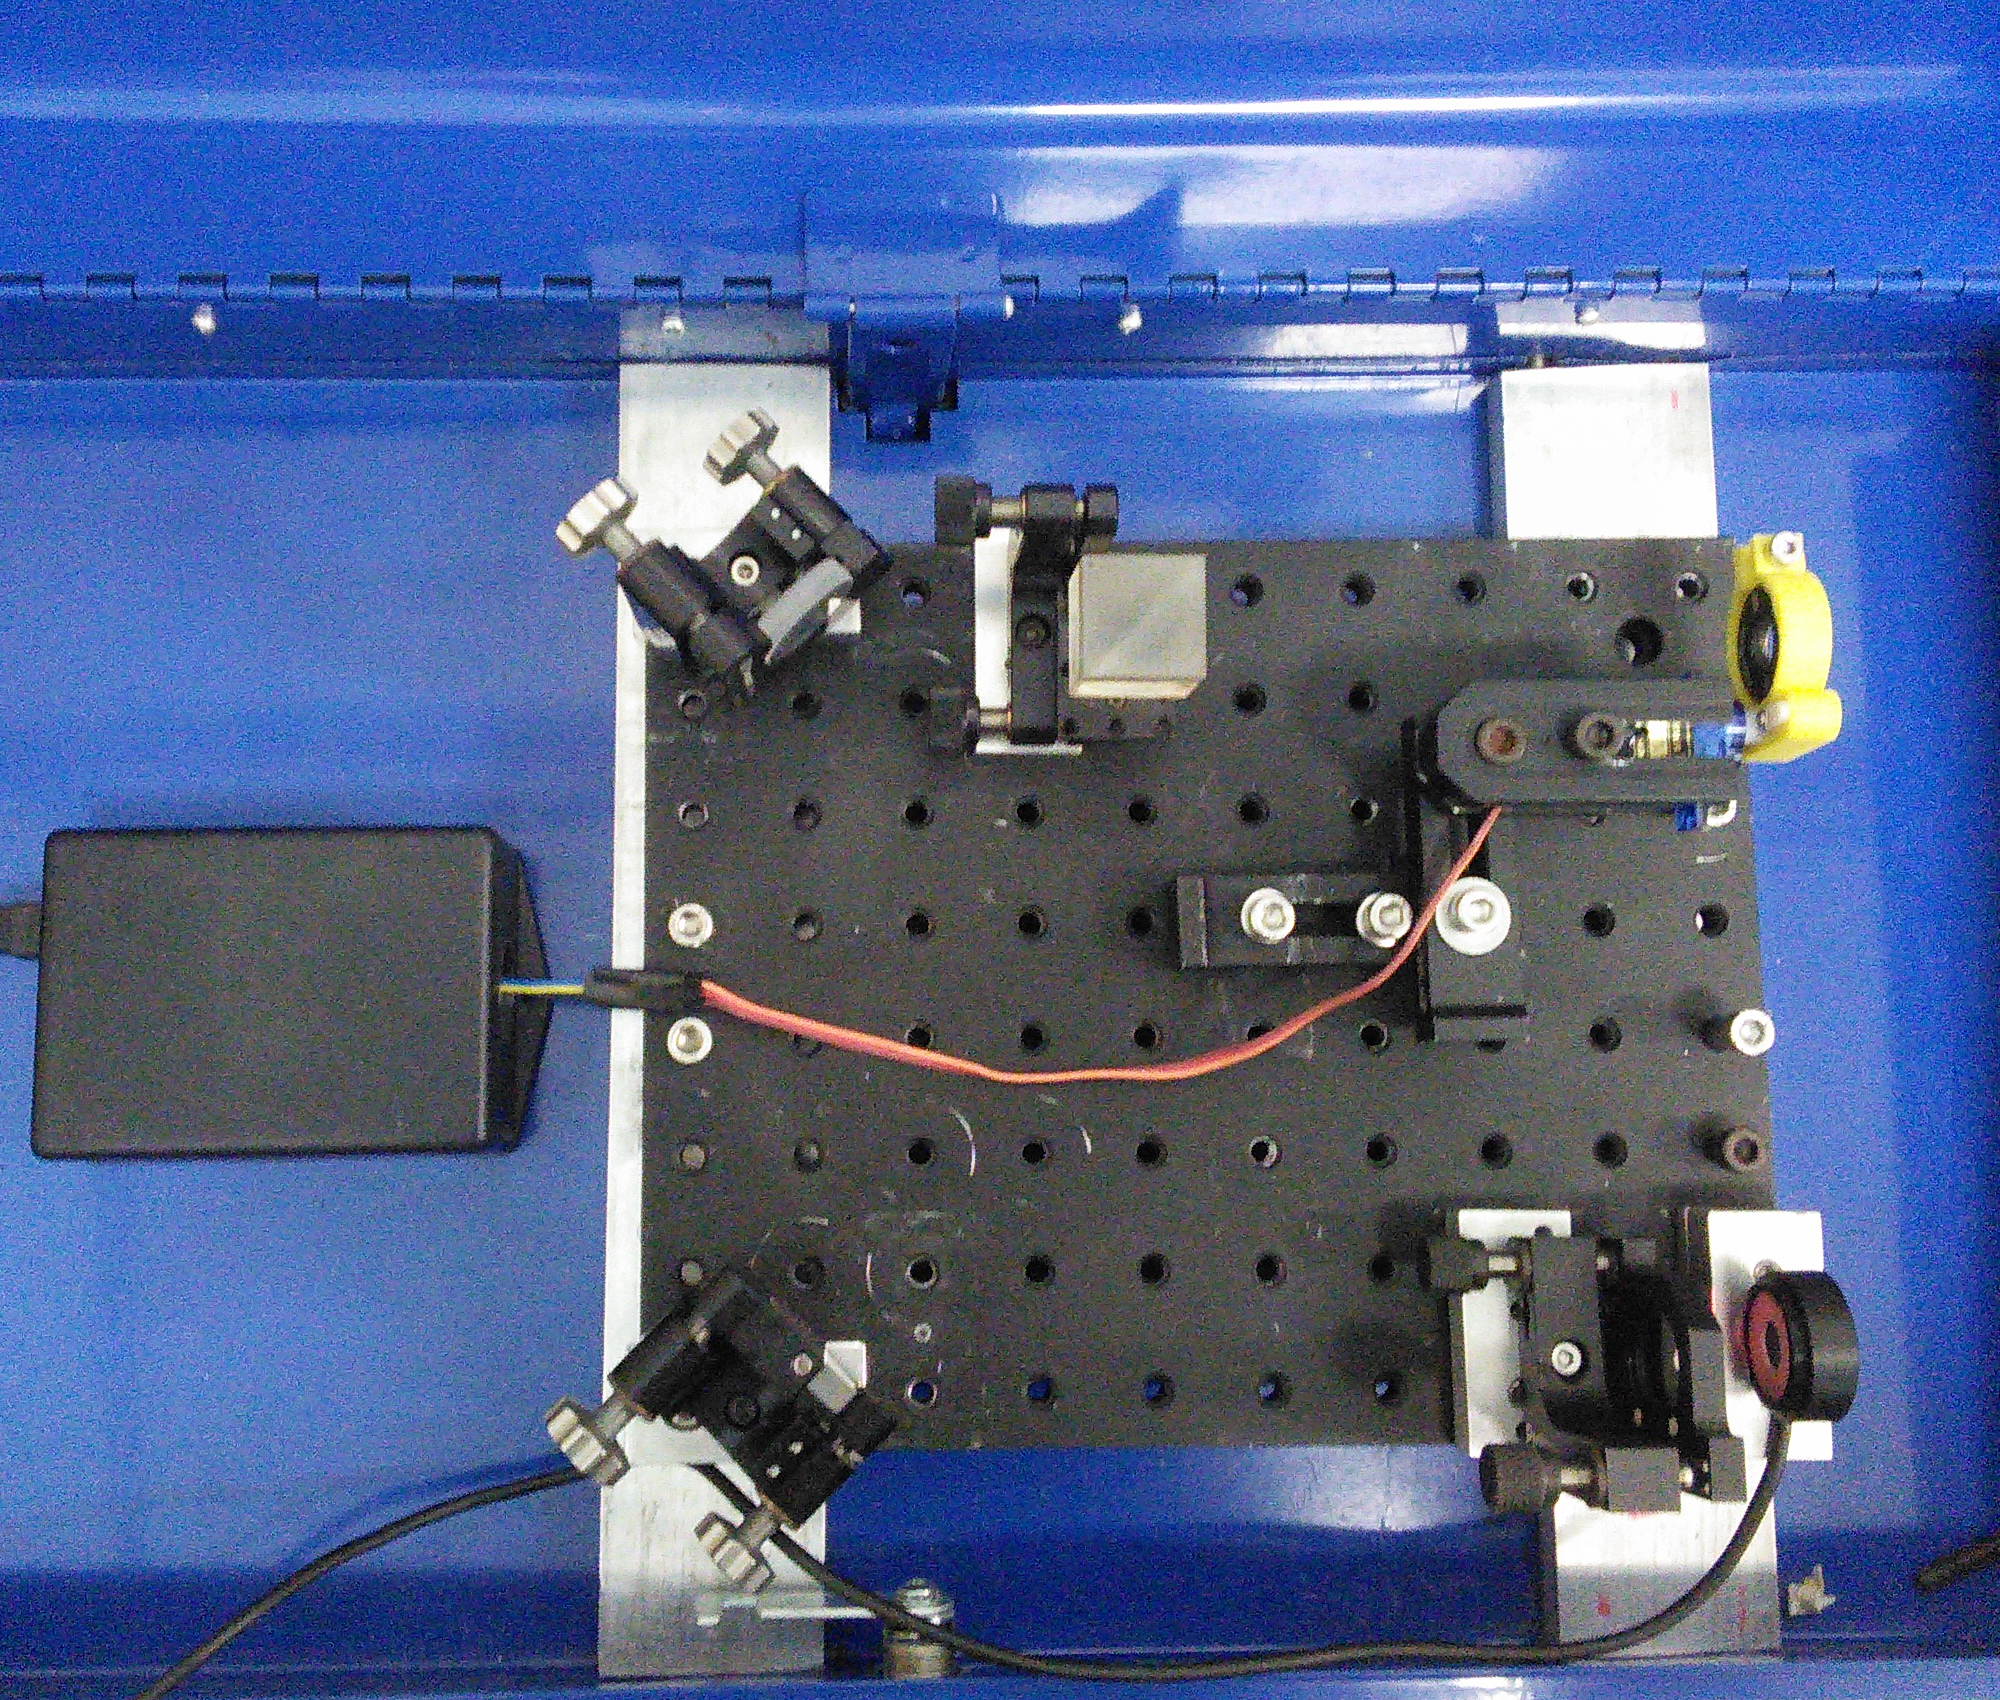
\includegraphics[width=15cm]{bob}
\hspace{0.5cm}
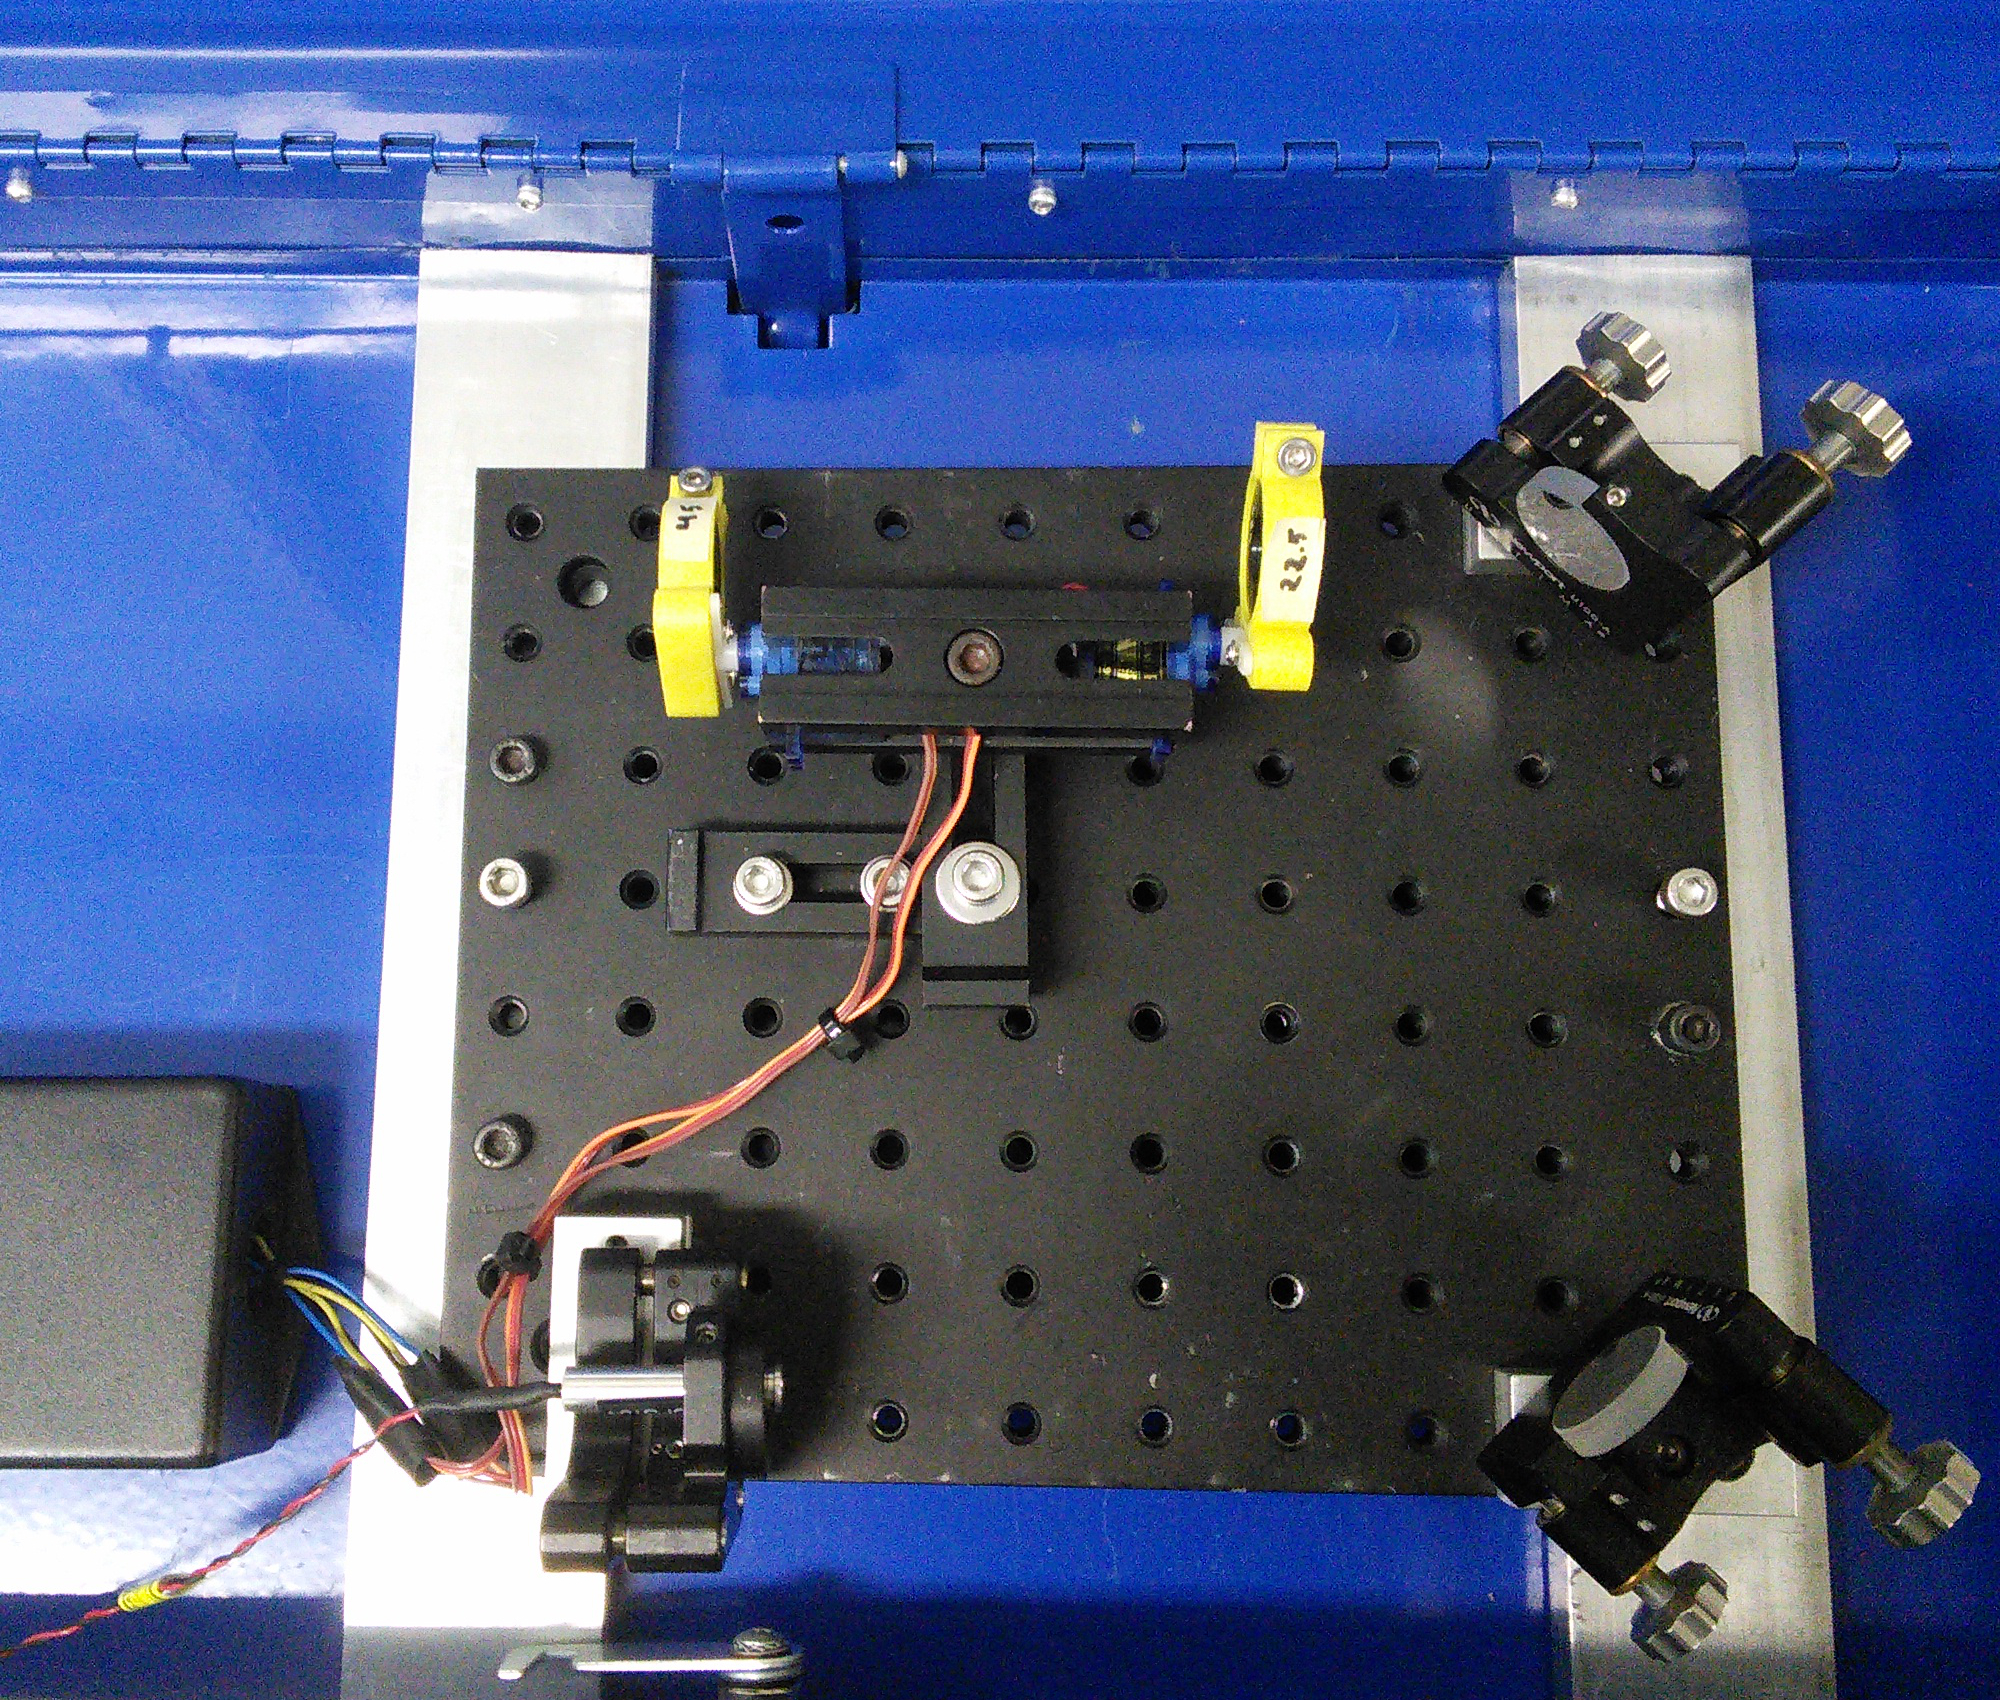
\includegraphics[width=15cm]{alice}

\vspace{1cm}
\hspace{8.75cm}
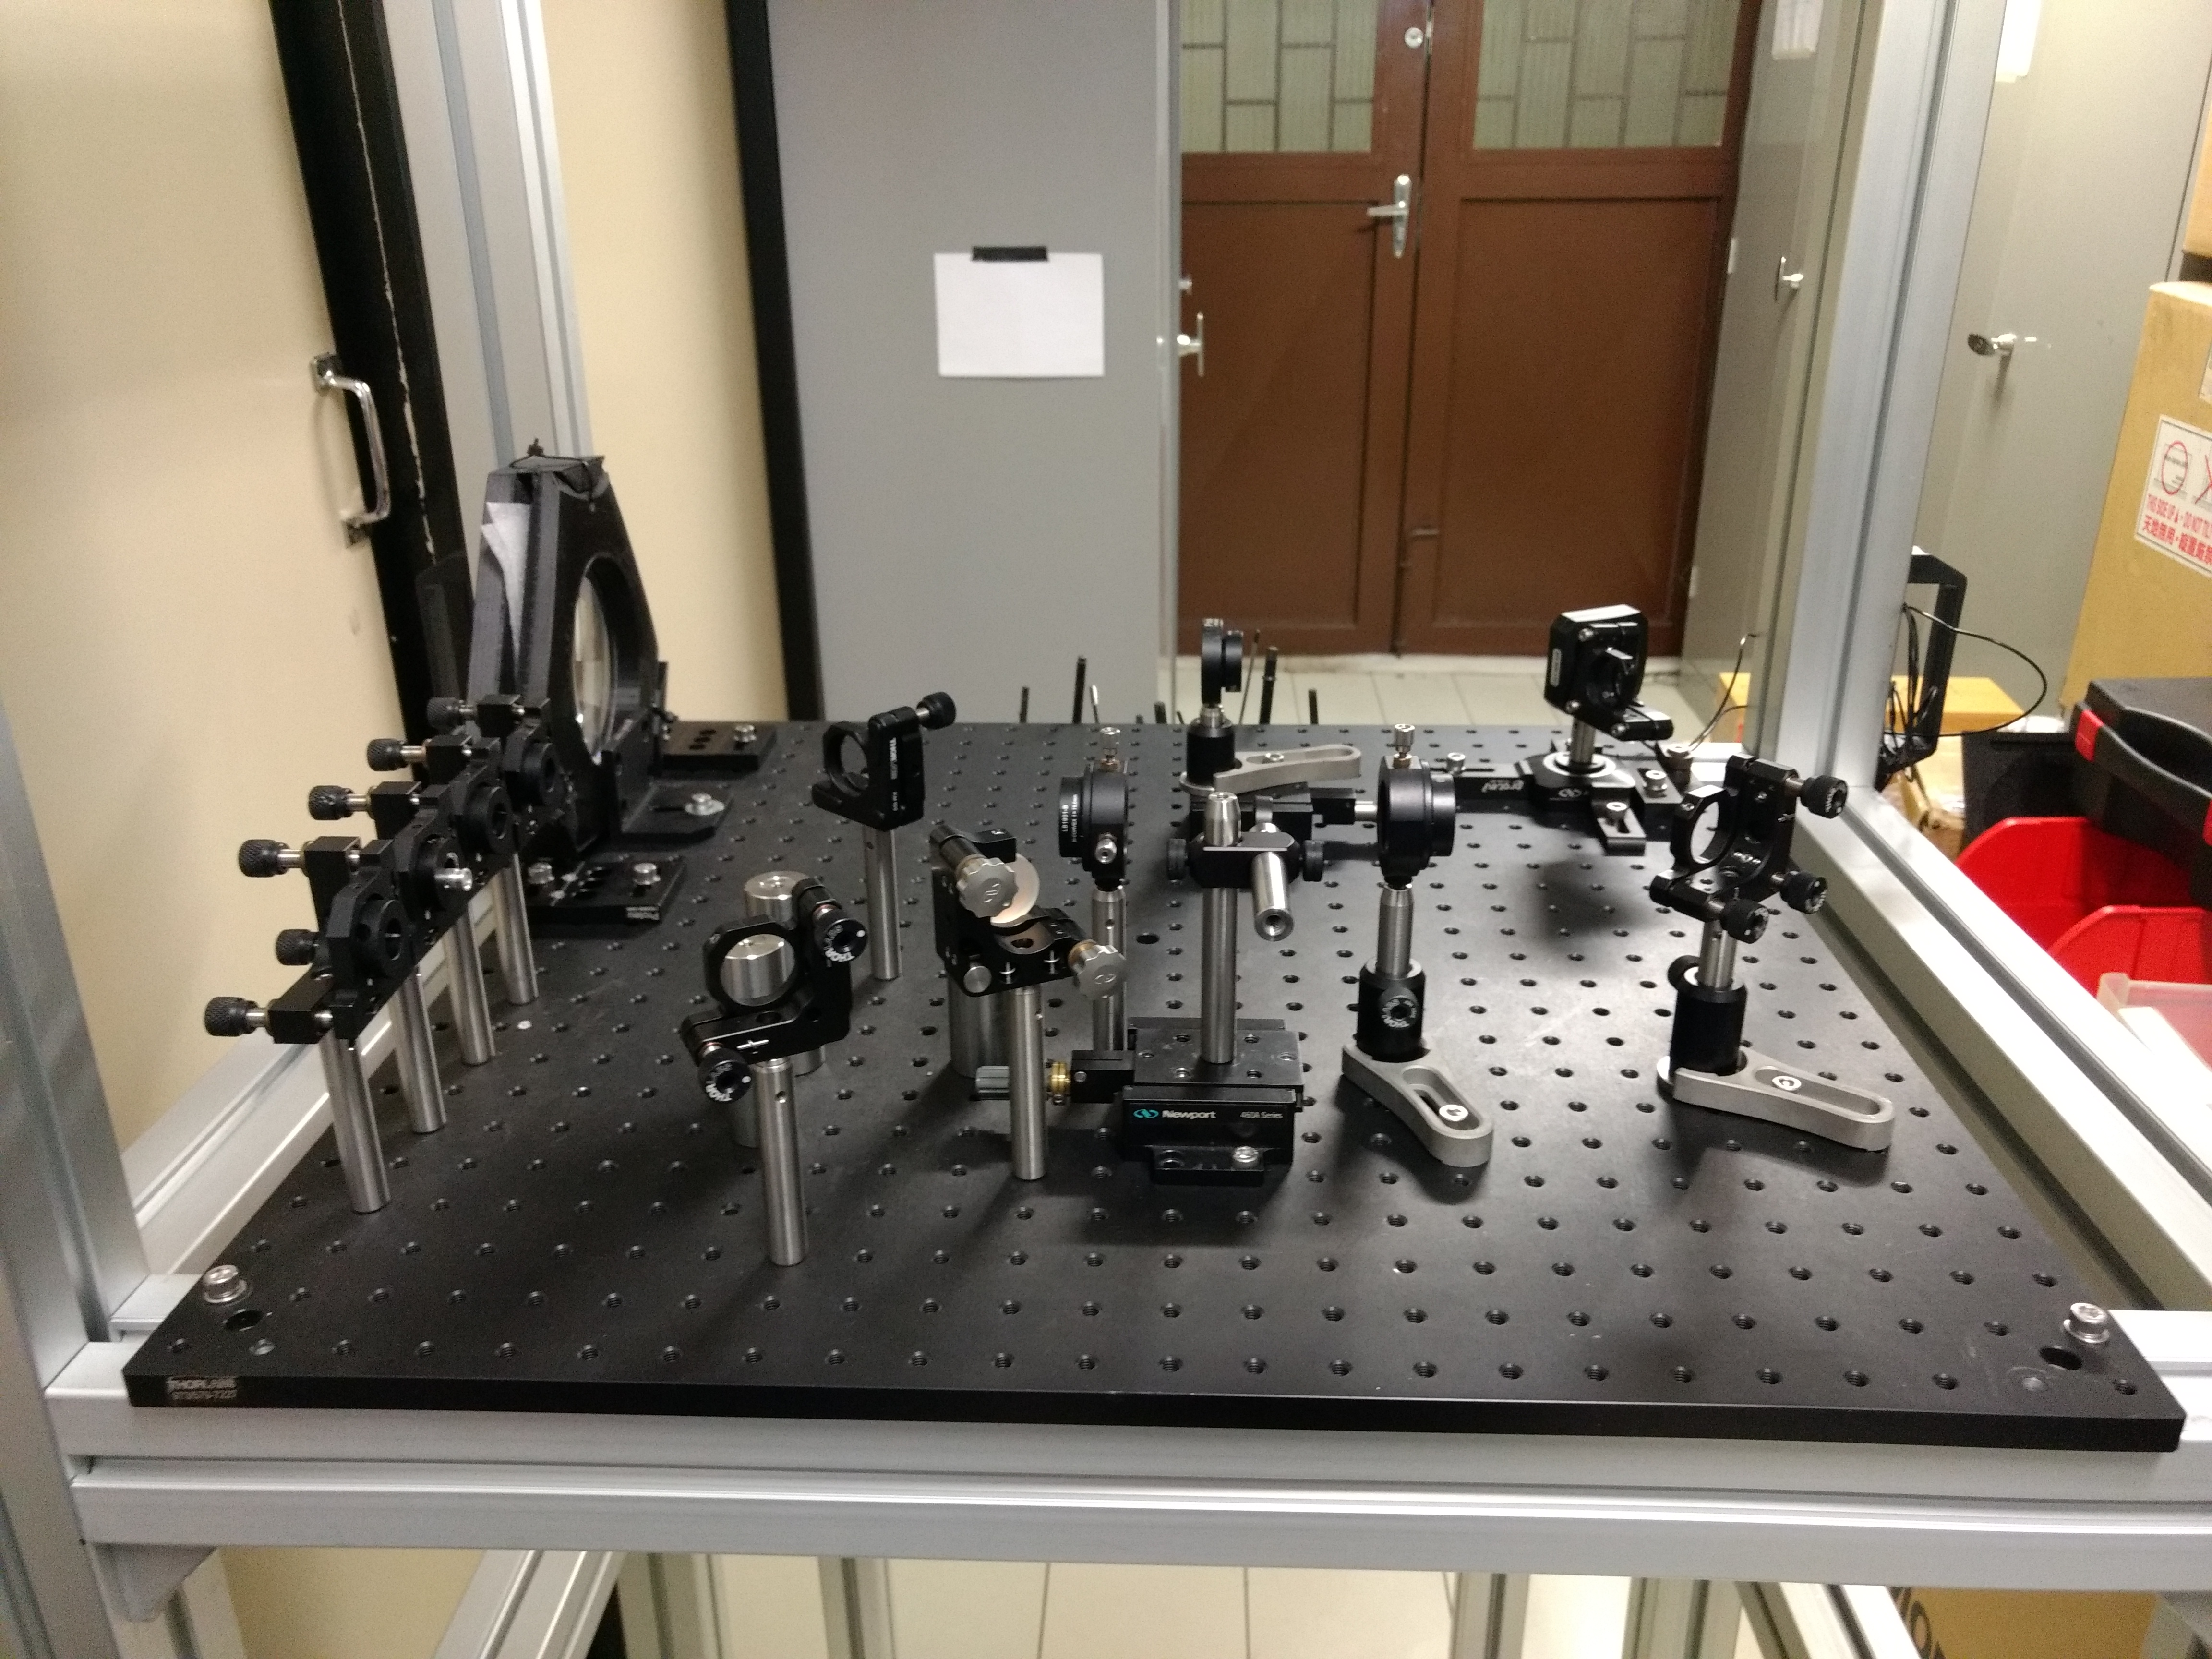
\includegraphics[width=15cm]{new_alice}



\section*{\tituloA{\color{white}{\large{Ao Infinito e Além!}}}}

\par Realizando uma rápida pesquisa na internet, encontramos facilmente diversos centros de pesquisas especializados e até mesmo empresas explorando criptografia quântica a nível comercial em diversos lugares do mundo. No Brasil, no entanto, pouco se fala a respeito do assunto e o conhecimento técnico da área é muito limitado.
\par Nosso estudos buscam, assim, gerar experiência e desenvolvimento nacional e, junto ao efervescente cenário brasileiro de segurança da informação, tornar o Brasil uma referêrencia na área.


}
\end{multicols*}



\end{document}
